% Options for packages loaded elsewhere
\PassOptionsToPackage{unicode}{hyperref}
\PassOptionsToPackage{hyphens}{url}
%
\documentclass[
]{article}
\usepackage{lmodern}
\usepackage{amssymb,amsmath}
\usepackage{ifxetex,ifluatex}
\ifnum 0\ifxetex 1\fi\ifluatex 1\fi=0 % if pdftex
  \usepackage[T1]{fontenc}
  \usepackage[utf8]{inputenc}
  \usepackage{textcomp} % provide euro and other symbols
\else % if luatex or xetex
  \usepackage{unicode-math}
  \defaultfontfeatures{Scale=MatchLowercase}
  \defaultfontfeatures[\rmfamily]{Ligatures=TeX,Scale=1}
\fi
% Use upquote if available, for straight quotes in verbatim environments
\IfFileExists{upquote.sty}{\usepackage{upquote}}{}
\IfFileExists{microtype.sty}{% use microtype if available
  \usepackage[]{microtype}
  \UseMicrotypeSet[protrusion]{basicmath} % disable protrusion for tt fonts
}{}
\makeatletter
\@ifundefined{KOMAClassName}{% if non-KOMA class
  \IfFileExists{parskip.sty}{%
    \usepackage{parskip}
  }{% else
    \setlength{\parindent}{0pt}
    \setlength{\parskip}{6pt plus 2pt minus 1pt}}
}{% if KOMA class
  \KOMAoptions{parskip=half}}
\makeatother
\usepackage{xcolor}
\IfFileExists{xurl.sty}{\usepackage{xurl}}{} % add URL line breaks if available
\IfFileExists{bookmark.sty}{\usepackage{bookmark}}{\usepackage{hyperref}}
\hypersetup{
  pdftitle={Simulation results},
  pdfauthor={Ella Orme},
  hidelinks,
  pdfcreator={LaTeX via pandoc}}
\urlstyle{same} % disable monospaced font for URLs
\usepackage[margin=1in]{geometry}
\usepackage{graphicx}
\makeatletter
\def\maxwidth{\ifdim\Gin@nat@width>\linewidth\linewidth\else\Gin@nat@width\fi}
\def\maxheight{\ifdim\Gin@nat@height>\textheight\textheight\else\Gin@nat@height\fi}
\makeatother
% Scale images if necessary, so that they will not overflow the page
% margins by default, and it is still possible to overwrite the defaults
% using explicit options in \includegraphics[width, height, ...]{}
\setkeys{Gin}{width=\maxwidth,height=\maxheight,keepaspectratio}
% Set default figure placement to htbp
\makeatletter
\def\fps@figure{htbp}
\makeatother
\setlength{\emergencystretch}{3em} % prevent overfull lines
\providecommand{\tightlist}{%
  \setlength{\itemsep}{0pt}\setlength{\parskip}{0pt}}
\setcounter{secnumdepth}{-\maxdimen} % remove section numbering
\usepackage{booktabs}
\usepackage{longtable}
\usepackage{array}
\usepackage{multirow}
\usepackage{wrapfig}
\usepackage{float}
\usepackage{colortbl}
\usepackage{pdflscape}
\usepackage{tabu}
\usepackage{threeparttable}
\usepackage{threeparttablex}
\usepackage[normalem]{ulem}
\usepackage{makecell}
\usepackage{xcolor}

\title{Simulation results}
\author{Ella Orme}
\date{}

\begin{document}
\maketitle

\hypertarget{resnmtf}{%
\section{ResNMTF}\label{resnmtf}}

\begin{figure}[H]

{\centering 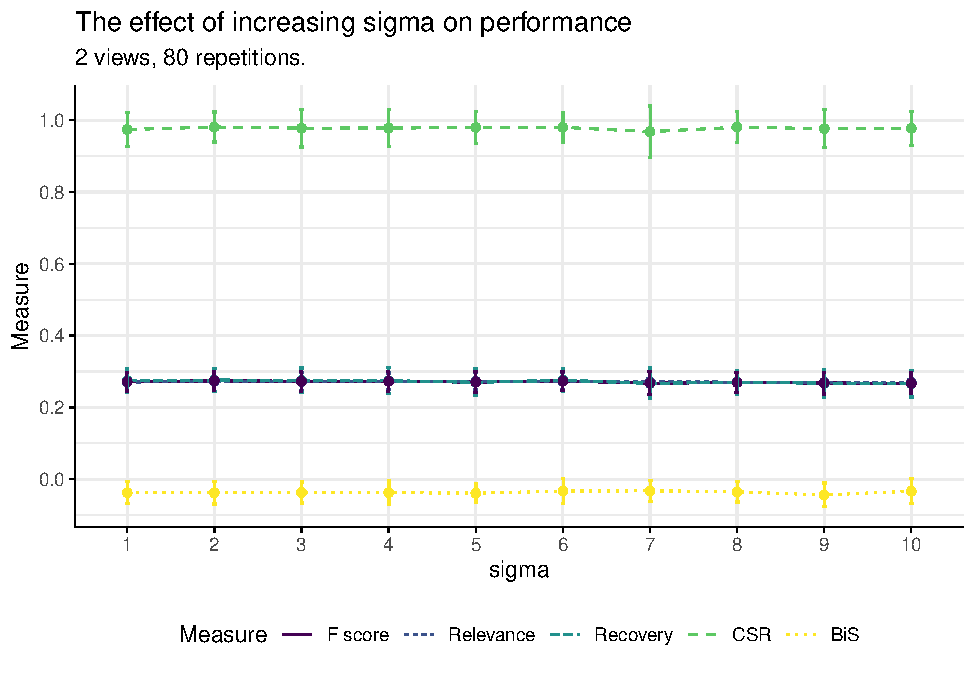
\includegraphics{issvd_results_files/figure-latex/unnamed-chunk-3-1} 

}

\caption{Simulation results for ResNMTF only.}\label{fig:unnamed-chunk-3}
\end{figure}

\begin{table}
\centering
\begin{tabular}[t]{llllllllllllllllllllll}
\toprule
\multicolumn{1}{c}{ } & \multicolumn{21}{c}{Per-comparrison wise error rate} \\
\cmidrule(l{3pt}r{3pt}){2-22}
  & 0 & 0.05 & 0.1 & 0.15 & 0.2 & 0.25 & 0.3 & 0.35 & 0.4 & 0.45 & 0.5 & 0.55 & 0.6 & 0.65 & 0.7 & 0.75 & 0.8 & 0.85 & 0.9 & 0.95 & 1\\
\midrule
F score & 0.0000 (0.0000) & 0.0000 (0.0000) & 0.0000 (0.0000) & 0.0000 (0.0000) & 0.0000 (0.0000) & 0.0000 (0.0000) & 0.0000 (0.0000) & 0.0000 (0.0000) & 0.0000 (0.0000) & 0.0000 (0.0000) & 0.0000 (0.0000) & 0.0000 (0.0000) & 0.0000 (0.0000) & 0.0000 (0.0000) & 0.0000 (0.0000) & 0.0000 (0.0000) & 0.0000 (0.0000) & 0.0000 (0.0000) & 0.0000 (0.0000) & 0.0000 (0.0000) & 0.0000 (0.0000)\\
Relevance & 0.0000 (0.0000) & 0.0000 (0.0000) & 0.0000 (0.0000) & 0.0000 (0.0000) & 0.0000 (0.0000) & 0.0000 (0.0000) & 0.0000 (0.0000) & 0.0000 (0.0000) & 0.0000 (0.0000) & 0.0000 (0.0000) & 0.0000 (0.0000) & 0.0000 (0.0000) & 0.0000 (0.0000) & 0.0000 (0.0000) & 0.0000 (0.0000) & 0.0000 (0.0000) & 0.0000 (0.0000) & 0.0000 (0.0000) & 0.0000 (0.0000) & 0.0000 (0.0000) & 0.0000 (0.0000)\\
Recovery & 0.0000 (0.0000) & 0.0000 (0.0000) & 0.0000 (0.0000) & 0.0000 (0.0000) & 0.0000 (0.0000) & 0.0000 (0.0000) & 0.0000 (0.0000) & 0.0000 (0.0000) & 0.0000 (0.0000) & 0.0000 (0.0000) & 0.0000 (0.0000) & 0.0000 (0.0000) & 0.0000 (0.0000) & 0.0000 (0.0000) & 0.0000 (0.0000) & 0.0000 (0.0000) & 0.0000 (0.0000) & 0.0000 (0.0000) & 0.0000 (0.0000) & 0.0000 (0.0000) & 0.0000 (0.0000)\\
CSR & 0.1429 (0.0000) & 0.1429 (0.0000) & 0.1429 (0.0000) & 0.1429 (0.0000) & 0.1429 (0.0000) & 0.1429 (0.0000) & 0.1429 (0.0000) & 0.1429 (0.0000) & 0.1429 (0.0000) & 0.1429 (0.0000) & 0.1429 (0.0000) & 0.1429 (0.0000) & 0.1429 (0.0000) & 0.1429 (0.0000) & 0.1429 (0.0000) & 0.1429 (0.0000) & 0.1429 (0.0000) & 0.1429 (0.0000) & 0.1429 (0.0000) & 0.1429 (0.0000) & 0.1429 (0.0000)\\
BiS & 0.0000 (0.0000) & 0.0000 (0.0000) & 0.0000 (0.0000) & 0.0000 (0.0000) & 0.0000 (0.0000) & 0.0000 (0.0000) & 0.0000 (0.0000) & 0.0000 (0.0000) & 0.0000 (0.0000) & 0.0000 (0.0000) & 0.0000 (0.0000) & 0.0000 (0.0000) & 0.0000 (0.0000) & 0.0000 (0.0000) & 0.0000 (0.0000) & 0.0000 (0.0000) & 0.0000 (0.0000) & 0.0000 (0.0000) & 0.0000 (0.0000) & 0.0000 (0.0000) & 0.0000 (0.0000)\\
\bottomrule
\multicolumn{22}{l}{\textsuperscript{a} 3 views, 100 repetitions.}\\
\end{tabular}
\end{table}

\hypertarget{correlation}{%
\section{Correlation}\label{correlation}}

\begin{tabular}[t]{lrr}
\toprule
  & BiS & CSR\\
\midrule
F score & NA & NA\\
Relevance & NA & NA\\
Recovery & NA & NA\\
\bottomrule
\end{tabular}

\end{document}
